% PART 1
\chapter{De-identification}
\label{ch:de-identification}
\startchapter

% segue (Removed: Adds nothing)
% The last chapter introduced a protocol for data provenance that serves as the basis for describing and constructing computational pipelines for analysing sport data. In sport, while some processes can be automated, the nature of sport analysis is such that some processes (e.g. observing video) are likely to be manual for the foreseeable future (e.g. until such a time as computer vision recognition can reliably label events in video images at an accuracy comparable to a human). Thus it was important that the proposed data provenance framework could manage the interplay between both automated and manual tasks.

% The last chapter also noted that there were some tasks, such as data de-identification, where certain kinds of data provenance should \textit{not} be possible. Specifically, the purpose of de-identification is to ensure that once data are de-identified, the results cannot be traced back to the individual participant the data relate to.

% \isec{How this chapter relates to rest of thesis}

The background chapter outlined the shift from traditional sport statistics that summarise game events towards detailed spatio-temporal datasets that track the position of every player on the team, at each moment, in high fidelity.

The increase in the volume and detail of data creates an opportunity for deeper forms of analysis than traditional approaches. However, the level of detail also raises new concerns about the risk of harm to player privacy, particularly when these datasets are shared with external parties outside of clubs, resulting in the potential for the dataset to be used in ways that are contrary to the wishes of players.

Typically, this is solved by the data custodian (the football club) de-identifying player tracking data (e.g. substituting player names with randomised anonymous codes) prior to handing the dataset over for use in research. However, the level of detail involved in player tracking datasets means that even after known identifiers are removed, there is often sufficient auxiliary information left in the dataset to re-identify players.

If data is collected for club use only, and players consent to the data collection, then de-identification may not be necessary when the analysis is all conducted in-house by trusted sport performance analysts working at the club. In contrast, this chapter deals with the situation where clubs share the data with an external party, such as a sport researcher outside of the club. In such a case, players may be unwilling to share their data in identifiable form, or the data may relate to former players who consented to sharing identifiable data within the club, but cannot be practically contacted anymore to seek approval to reuse their data in new ways. In this situation, it is vital that the data be properly de-identified to protect the players' privacy rights.

This chapter explores the issues surrounding de-identification of detailed sport datasets, in particular GPS player tracking data and associated datasets. As noted in the previous chapter introducing computational pipelines, de-identification is a form of data transformation operation that can be considered as part of the overall pipeline. % De-identification should ideally occur as early in the pipeline as possible to reduce the risk of exposing private information in later stages of the pipeline.

The de-identification operation has special considerations that distinguish it from other components of the pipeline. Unlike other operations where it is desirable to have a means to trace the provenance of results back to records in the underlying dataset, the aim of data de-identification is to ensure that results \textit{cannot} be traced back to the individual the data relate to. As such, the de-identification operation must be under the control of the data custodian, as only the data custodian should have access to the original underlying identifiable data. However, sport researchers external to the club need to be able to design and run operations that form the rest of the computational pipeline acting upon the de-identified data. This motivates the design of an new interaction model for de-identification of human data.

This chapter is directly applicable to sport research involving de-identification of spatio-temporal data. The interaction model presented is also applicable to other fields where researchers require access to detailed human data in non-identifiable form but the data custodian has limited technical resources to carry out the de-identification process. The findings of this chapter informed the design of the de-identification process used to obtain the non-identifiable datasets used throughout this thesis.

\section{Introduction}

A machine learning approach to sport analysis requires access to detailed data about each action in the match, % to train the model,
as opposed to traditional sport statistics that deal only with summary statistics about the match. In the statistics literature, detailed datasets containing individual rows for each participant (i.e. the players) are known as \textit{microdata}.

%detailed datasets containing individual rows for each participant (i.e. the players) rather than summaries are said to contain \textit{microdata}.
%(technically "contain microdata" is more accurate, but makes microdata term cumbersome to use later on)

% From low risk ethics application:
% Although AFL matches are played in public and standard player contracts permit use of ``data utilised for player position and team'' \footnote{AFL, ``Use of Player Information -- Clubs'' In ``Collective Bargaining Agreement 2017 -- 2022 Australian Football League'', Section 45.3. Available: \url{http://www.aflplayers.com.au/cba/}}, there have been media reports that the AFL Players' Association (AFLPA) is concerned that ``footballers will face heightened scrutiny if an AFL plan to provide in-game player GPS tracking data to broadcasters comes to fruition.'' \footnote{The Age, ``AFLPA raises concerns about plan for broadcasters to show AFL player GPS data'', 9 Feb 2017. Available: \url{https://www.theage.com.au/sport/afl/aflpa-raises-concerns-about-plan-for-broadcasters-to-show-afl-player-gps-data-20170209-gu9jtr.html}}

However, microdata introduces legal and ethical concerns:

\begin{enumerate}

\item Although sport matches are played in public, there are concerns from players and player representation bodies about the unprecedented level of individual player scrutiny that could occur as a result of in-match player tracking.\footnote{The Age, ``AFLPA raises concerns about plan for broadcasters to show AFL player GPS data'', 9 Feb 2017. Available: \url{https://www.theage.com.au/sport/afl/aflpa-raises-concerns-about-plan-for-broadcasters-to-show-afl-player-gps-data-20170209-gu9jtr.html}}

\item Human research ethics codes encourage researchers to de-identify data where possible. Ethics exemption may be granted for use of pre-existing non-identifiable data, whereas cases where data are identifiable or re-identifiable (and not already public) require participant consent and/or justification that the befits of the research outweigh the risk of harm to participant privacy.

\end{enumerate}

De-identification is a one-off transformation that should be applied to the data as early as possible, preferably by the data custodian prior to release of data. While stripping identifying information or replacing it with random anonymous identifiers may at first seem trivial, this chapter shows that de-identifying data in a way that preserves privacy against attack is non-trivial, and the proper choice of procedure should be informed by the nuances of the domain. In particular, an ideal state is to prevent the ability to re-identify individual players based on player movement or scoring profiles, while preserving the ability to perform high-level/aggregate analysis (e.g. spatio-temporal analysis of team formations).

As the aim of sport research is to capture generalisable patterns rather than critique individuals, and considering the legal and ethical concerns surrounding data that could identify individuals, the data should undergo a de-identification process as early as possible. However, the de-identification of high-dimensional microdata is challenging to perform in a way that is secure against all possible re-identification attacks. Furthermore, these issues are exasperated for spatio-temporal data (discussed in \secref{sec:deidentification-of-spatial-data} and \secref{sec:de-identification-methods-gps}).

The work presented in this chapter was motivated and shaped by a series of interactions that showed systematic gaps between the theoretical privacy rights of participants in research and the state of sport research in practice. The project involved interaction with sport performance analysts at two elite sport organisations. The first club provided identifiable GPS data, without any discussion regarding player consent, nor data confidentiality beyond goodwill.\footnote{The analysis presented in \chref{ch:integration} does not use data from this club.} Communicating with a sport practitioner at the other club, they provided a sample of identifiable possession chain data for one match.\footnote{This sample of possession chain data was not used as part of analysis in \chref{ch:integration} either.} While greatly appreciative of the trust of both of these clubs, particularly the collegiality of individuals at the clubs without whom this research project would not have been possible, these actions are suggestive of the current attitudes towards data sharing by sport practitioners; i.e. a culture of data sharing based on goodwill and relationships between researchers and sport practitioners, rather than on the consent of the individuals to whom the data pertains.

Furthermore, there were projects in university research centres that used de-identification schemes that were fundamentally flawed, such as anonymous identifiers generated through a deterministic rather than random process, or included a large number of auxiliary attributes that could be linked to identifiable information. These projects often stated data as being ``non-identifiable'' in ethics applications and were approved without further question. These personal observations triggered a deeper investigation to confirm whether these experiences are part of a more general phenomenon. % outside of projects we have been involved with
The presentation of this investigation aims to bring the advances in understanding of privacy that have occurred in the computer science domain to the sport research domain.

This chapter:
\begin{enumerate}
  \item Reviews the literature on formal methods and best practices for de-identification of research data sets.
  \item Studies a sample of sport research papers to establish common de-identification issues faced by sport researchers and practitioners.
  \item Considers re-identification risks for player position tracking data, with the goal of identifying a de-identification method that preserves player privacy without destroying the utility of the data for team-level spatio-temporal analysis.
  %\item Presents a de-identification model. % supervisor: worth making this explicit
  \item Provides an interaction model for requesting datasets with special de-identification requirements from external data custodians without revealing the underlying raw data.
  \item Applies this work through a case study in de-identification of \afl{} player tracking datasets.
\end{enumerate}

% \isec{Importance of proper de-identification}

\subsection{Large scale privacy breaches due to improper de-identification}

The below list shows examples of large scale privacy breaches of private and government released microdata due to improper de-identification methodologies. Note that none of these were due to conventional cyber-attacks, but rather due to deliberately released datasets without a proper understanding of the risks of re-identification. These have been reported in the literature \cite{Ohm2010, ElEmam2011} and media:

\begin{enumerate}
\item 1997: Massachusetts Group Insurance Commission (GIC) releases de-identified health insurance data. Sweeny \cite{Sweeny2002} later shows that the health records can be linked to the voter registration list on ZIP code (postcode), sex, and date of birth to re-identify individuals, using the governor of Massachusetts at the time as an example.  % (sweeny, cited by ohm)
\item 2006: AOL releases search data, substituting user identifiers with anonymous codes. However, as searches conducted by the same user shared the same anonymous code, it was possible to use keywords in their search terms to build up a profile on their likely location and identity, eventually culminating in a confirmed re-identification.\footnote{The New York Times, ``A Face Is Exposed for AOL Searcher No. 4417749'' \url{https://www.nytimes.com/2006/08/09/technology/09aol.html}, 9 Aug 2006} % [https://epic.org/privacy/reidentification/] (cited by ohm)
\item 2006: Netflix releases de-identified user movie ratings, challenging data scientists to come up with a better movie recommendation algorithm. The dataset is later taken down after researchers reveal that knowledge of three movie ratings for a user (e.g. obtained from external movie review sites or by asking in person), and the approximate dates the movies were rated, is enough to uniquely identify the Netflix user with 80\% probability. This results in revealing viewing history of other movies that the user did not intend to be publicly associated with \cite{Narayanan2008}. % [https://epic.org/privacy/reidentification/] (cited by ohm)
\item 2016: Australian Department of Health releases de-identified medical billing records to \url{data.gov.au}, the Australian Open Data portal. The dataset is later taken down after researchers discover that the algorithm to generate unique anonymous identifiers is fundamentally flawed due to the use of a deterministic rather than random generation procedure. Knowledge of a few medical billing records (such as dates of baby delivery, or publicly reported medical conditions) is sufficient to re-identify individuals in the dataset and thus learn their full medical billing history which may reveal private information of a more sensitive nature \cite{Culnane2017}.
\end{enumerate}
%  non-publicly known medical inform records for those individuals, such as medical billing those of a more sensitive nature

% While the failures of de-identification of past decades could be partially excused on the basis of insufficient understanding at the time, the recent failure by Australian Department of Health in 2016 suggests systematic issues.

%\isec{Motivation}
%\subsubsection{Legal and ethical implications}
% Supervisor: Most of this is excellent to set stage as motivation, move up into introduction

In his seminal 2010 article, ``Broken Promises of Privacy: Responding to the Surprising Failure of Anonymization'' \cite{Ohm2010}, Paul Ohm, a professor of law, examines the failure of de-identification methods to meet human expectations of privacy, as well as the theoretical limits on achieving privacy without destruction of data utility. He concludes that %what he calls
the ``robust anonymization assumption'' that data can be fully de-identified without damaging the utility of the dataset is false. He explains that this has been a ``fundamental misunderstanding'' of policy makers who set out privacy law and regulations, which has resulted in either ``much less privacy than we have assumed'' (in the US), or unattainable standards (e.g. in the EU). He describes the ``accretion problem'' in which each re-identifiable dataset, even if non-privacy invading in itself, permits linkage of others, and warns against the potential for a ``database of ruin'', compromising the privacy of every individual, which comes closer with every information disclosure. The rest of his article speculates on legal reforms needed to defend against issues that will inevitably arise as a result of the impossibility of having both privacy and free information flow in a world where unprecedented levels of data are already publicly available for linkage.

%\isec{Summary}
% Supervisor: Stating the obvious and hence can omit (summary title) in prose

These incidents demonstrate that de-identification is non-trivial to perform correctly, and failure to anticipate current and future attacks against the de-identification strategy can result in irrevocable damage both to the privacy of the individuals they pertain to, and the reputation of those responsible for the datasets. The following section will explore formal methods and best practices to protect against re-identification.

% - Facebook? (NA, either already public, or identifying - no attempt made at making non-identifiable - other than social network example)




%\section{Literature review}
\section{Background}
\label{ch:ethics-background}

\subsection{Formal methods for de-identification}
% Supervisor: This is good as Background

% Supervisor: There are four broad methods of de-identification that apply to microdata - a grouped hierarchy is shown in \figref{fig:deident-taxonomy}. In this section, we discuss each of these and discuss current state of art???

\figref{fig:deident-taxonomy} provides an overview of formal de-identification methods for microdata that will be discussed in this section. The section begins by reviewing deterministic algorithms for non-interactive data privacy whereby the data custodian applies an algorithm to remove or coarsen data attributes then hands the data over to the researcher to analyse. It then briefly touches on differential privacy, a mathematical framework for reasoning about the privacy guarantees offered by probabilistic privacy methods that distort the data through noise dependant upon the query made of the data. Finally, it will review literature on de-identification of spatio-temporal datasets. Spatio-temporal datasets tend to resist formal mathematical guarantees of privacy due to the uniqueness of movement patterns.

\begin{figure}[h]
  \centering
  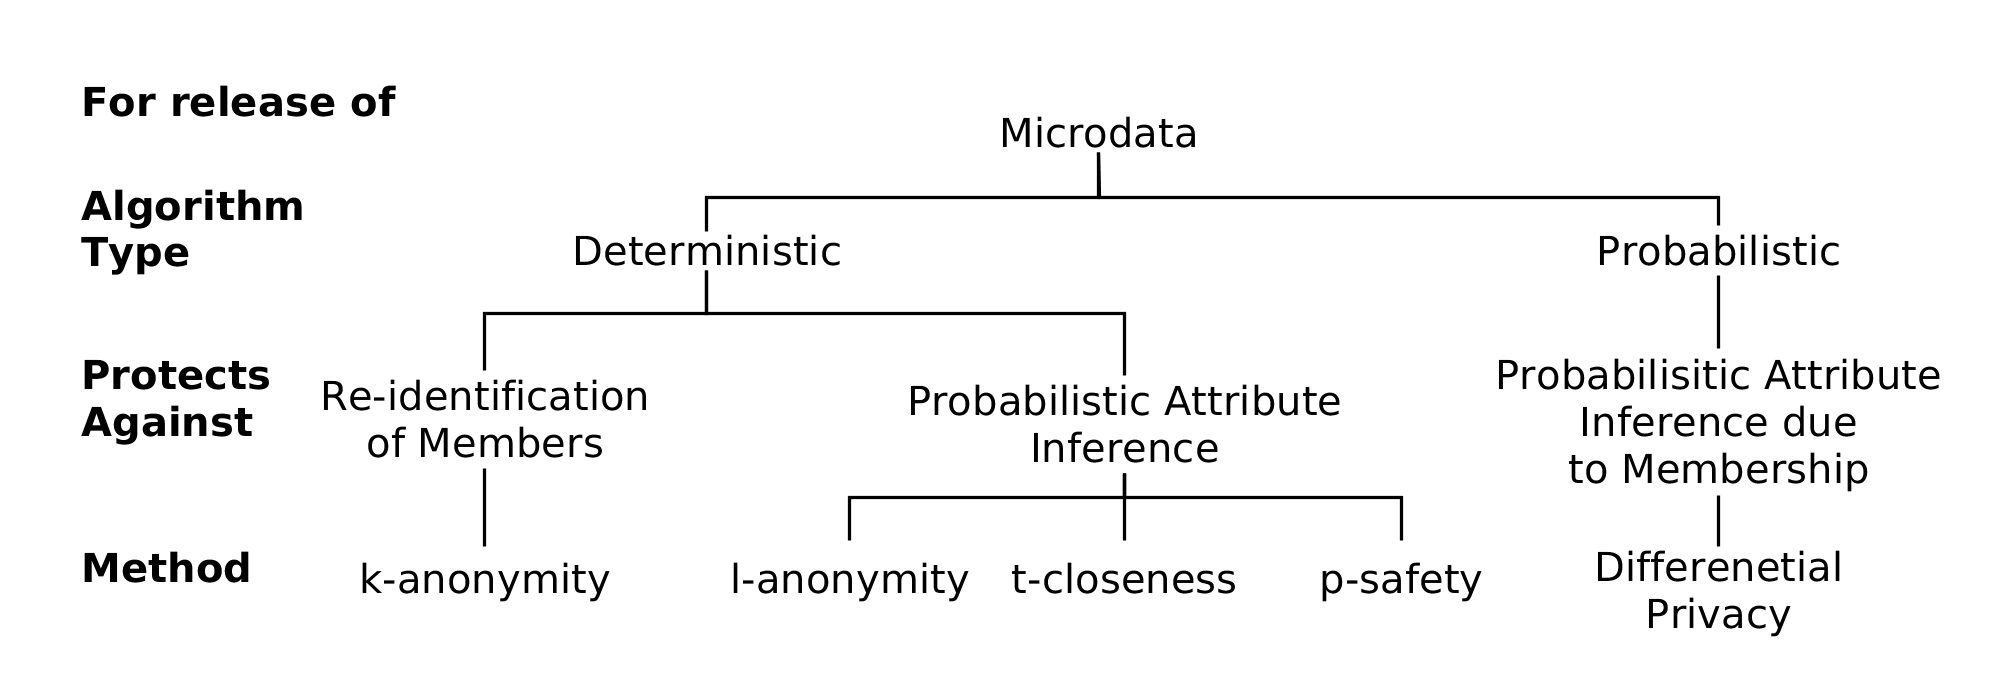
\includegraphics[width=\linewidth]{taxonomy1_v3}
  \caption{Taxonomy of formal de-identification methods}
  \label{fig:deident-taxonomy}
\end{figure}

% % Generated by https://www.tablesgenerator.com/
% \begin{table}[]
% \centering
% \caption{Taxonomy of formal de-identification methods}
% \label{tab:deident-taxonomy}
% \begin{tabular}{p{2.0cm}p{2.5cm}p{3.7cm}l}
% \hline
% \textbf{For \mbox{release} of}    & \textbf{Release Type}            & \textbf{Protects Against}                           & \textbf{Method}      \\ \hline
% \multirow{5}{*}{Microdata} & \multirow{4}{2.5cm}{Non-Interactive} & \mbox{Re-identification} of Members                        & \textit{k}-anonymity          \\ \cline{3-4}
%                            &                                  & \multirow{3}{3.7cm}{Probabilistic Attribute Inference}  & \textit{l}-diversity          \\ \cline{4-4}
%                            &                                  &                                                     & \textit{t}-closeness          \\ \cline{4-4}
%                            &                                  &                                                     & \textit{p}-safety             \\ \cline{2-4}
%                            & Interactive                      & Probabilistic Attribute Inference due to Membership & Differential Privacy \\ \hline
% \end{tabular}
% \end{table}

%\subsubsection{Non-interactive de-identification strategies for microdata}
\subsubsection{Deterministic de-identification strategies for microdata}

This section will examine measures and algorithms for de-identifying data. Specifically, it looks at deterministic strategies that generalise the data (e.g. by removing fields, reducing precision, or grouping into courser categories) without resorting to random distortion of the data (e.g. adding noise). Early de-identification methods proposed in the literature were later understood to suffer from certain forms of attacks, which motivated design of subsequent methods. To show the interplay between de-identification methods and re-identification attacks in the literature, a misuse case diagram (an adaptation of UML use case diagrams for the purpose of modelling threats \cite{Alexander2003}) displaying how the methods reviewed in this section build upon each other to correct previous limitations is presented in \figref{fig:misuse-case}.
% the interplay between de-identification methods and re-identification attacks in the literature
% To show how the methods reviewed in this section build upon each other to correct previous limitations

\begin{figure}[h]
  \centering
  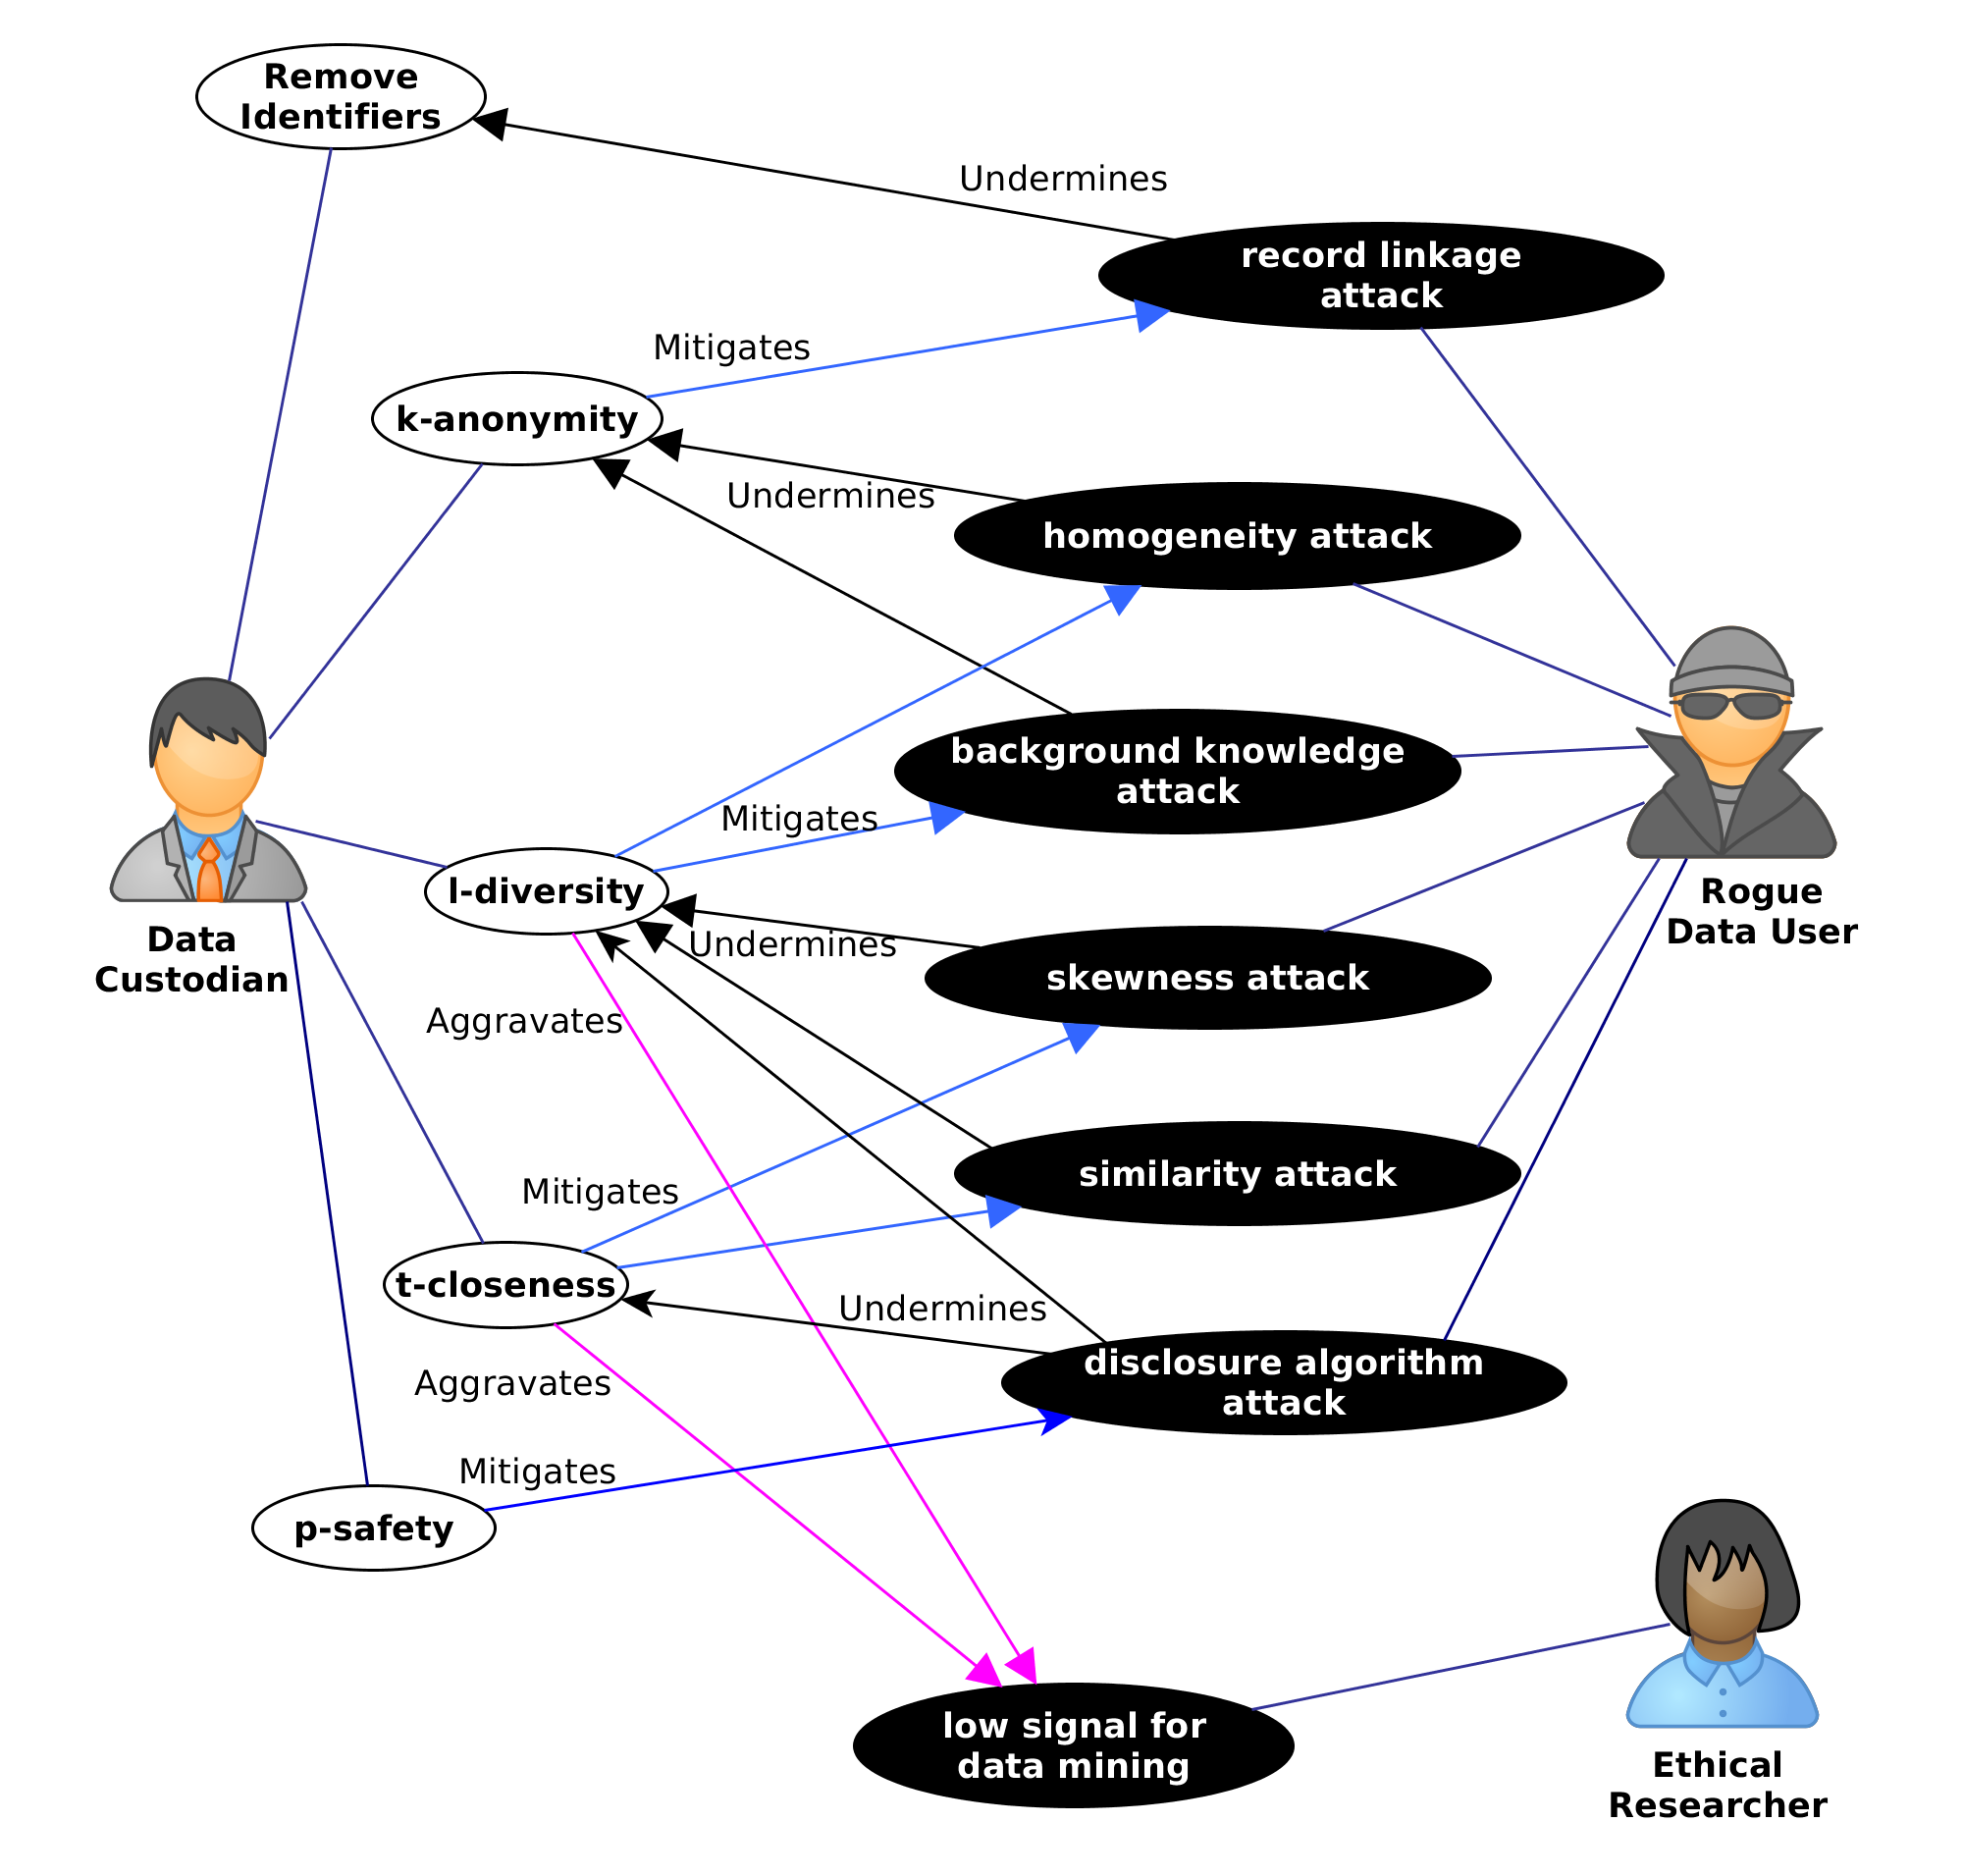
\includegraphics[width=\linewidth]{misuse-case-diagram-v5}
  \caption{Misuse case diagram showing attacks against non-interactive de-identification strategies for microdata}
  \label{fig:misuse-case}
\end{figure}

\paragraph{\textit{k}-anonymity}

Sweeny \cite{Sweeny2002} introduces the measure \textit{k}-anonymity as a tool to formally reason about resistance of a dataset to re-identification attacks based on uniqueness of attributes linkable to public data. Sweeny denotes the set of attributes potentially vulnerable to linkage as the \textit{quasi-identifier}. The level of \textit{k}-anonymity, \textit{k}, is defined as the minimum number of records that share the same \textit{quasi-identifier}. If $k>1$, then it is provably impossible to re-identify any particular player through record-linkage, as there will be multiple records sharing the same \textit{quasi-identifier} key (although the data may still be vulnerable to other forms of attack). If $k=1$, Sweeny considers the data to be potentially re-identifiable; however, this may be an overly conservative definition of privacy. Even if $k=1$ (which will always be the case if the dataset contains continuous attributes), the dataset is only re-identifable in practice if the attacker can obtain public data pertaining to the attributes of the \textit{quasi-identifier}, for the subjects the data pertains to, with enough precision to be confident in the linkage.

% For example, consider a publication that includes a scatter plot showing player height on the x-axis and a personal attribute such as player salary on the y-axis. As height is a continuous distribution, hight measurements are unique and thus the dataset does not meet the \textit{k}-anonymity criteria. However, in practice, an attacker is unlikely to be able to de-identify the data unless they can obtain high accuracy hight data for each of the players. While this is feasible at the elite level, for grass-root teams, the attacker's estimates of player heights (e.g. estimated from photographs) is unlikely to allow unique determination of player identities.

% While Sweeny's work offers a provable guarantee of resistance to linkage, it comes with caveats that may lead to \textit{k}-anonymity to be infeasible in practice.

Sweeny assumes that the data holder is able to determine the \textit{quasi-identifier}, i.e. the attributes vulnerable to data linkage. Sweeny provides the example that a quasi-identifier for medical data would include ZIP (postcode), birthdate, and sex, as these can be linked to voter lists. Sweeny also considers that the quasi-identifier should include other information an attacker may know, such as the patient's race. However, this task of understanding which details an attacker will have access to, is difficult in the current age, due to the micro-level information people publicly share about themselves online through social media and social networking tools. For example, Sweeny's example of de-identifying medical data assumes that the visit date of the medical appointment is unknown to the attacker, so does not need to be considered as part of the \textit{quasi-identifier}. However, with services such as Foursquare\footnote{Prior to removal of the Foursquare ``check in'' feature in 2014}, and Facebook, that encouraged users to share ``check ins'' to businesses, it is now feasible for an attacker to collect information such as visit date as a key to re-identify data. This is particularly problematic when de-identifying sport players' data, due to the pool of public information that could be used for a data linkage attack as a result of the public nature of both elite (via traditional media), and sub-elite (via social media) players' lives. For the case of sport match data de-identification, the presence of only % 22
a limited, known set of players on the team, and a large existing pool of identifiable data on each player, means that \textit{k}-anonymity is unlikely to be achievable.
% See also, Narayanan 2009, cited by Ohm: "We cannot predict the type and amount of outside information the adversary can access."
% narayana2014 - no-silver-bullet-de-identification.pdf - evidence of (heated) discussion in literature on practical implications.

% Supervisor: Gaps or limitations may be better presented at the end in AFL context?
% Associate Supervisor: disagrees (NO)

\paragraph{\textit{l}-diversity}

Machanavajjhala et al. \cite{Machanavajjhala2007} describe two attacks on \textit{k}-anonymity: the \textit{Homogeneity Attack}, and the \textit{Background Knowledge Attack}. The \textit{k}-anonymity criterion only specifies the crowd group size that an individual may hide in, and thus anyone in that group is indistinguishable from $k-1$ individuals, but does not place any restrictions on the diversity of the group in which one hides, thus it may be possible to infer an attribute of an individual in the group on the basis that all members of the group share that attribute. For example, grouping players by team ensures a high value of \textit{k} equal to the size of team, but if all players on the team anonymously admit to having taken illicit performance enhancing substances, then this still results in revealing sensitive information about individuals. This is known as a \textit{Homogeneity Attack}. The \textit{Background Knowledge Attack} requires that the attacker has some additional information about one of the participants, as is often the case in reality, e.g. they may know that a certain participant on the team \textit{didn't} take performance enhancing substances, or the performance enhancing substance was not of a particular type. This may allow the attacker to infer which members of the team \textit{did} take performance enhancing substances by ruling out certain possibilities, even when \textit{k}-anonymous data is not immediately revealed via a homogeneity attack.

To solve these issues, Machanavajjhala et al. propose \textit{l}-diversity that extends \textit{k}-anonymity to further ensure a given level of diversity within each group. There are multiple methods of describing the diversity, so they consider both \textit{Entropy l-diversity} (which had been previously discovered, but without a general framework to motivate it) and \textit{Recursive (c,l)-diversity} (which guarantees diversity by ensuring that the $l-1$ most likely sensitive values in each group each make up less than $c$ times the number of the remaining values in the group). % this is just a restatement of the formula provided in Machanavajjhala definition 4.2.
This means that an attacker would have to rule out at least $l-1$ other values or records in the group in order to confidently infer a sensitive attribute.
% as explained by Machanavajjhala, ruling out values is always equivalent to ruling out at least one record.
% Machanavajjhala: "the adversary needs to eliminate at least ...-1 possible
%                   values of S in order to infer a positive disclosure"
%

% Supervisor: An implementation ... is tested to show ...
% \as {Kept in active rather than passive voice. Need to make it clear that we are reporting other findings (thus need to mention/cite researcher) rather than claiming to have performed the experiment ourselves}.
% Machanavajjhala et al. tested an implementation of k-anonymity and show that a \textit{Homogeneity Attack} is often possible in practice. Furthermore, they show that the structure of \textit{k}-anonymity and \textit{l}-anonymity is similar enough that algorithms for rendering data \textit{k}-anonymous can easily be extended to also implement the \textit{l}-anonymity algorithm as a more stringent alternative option.

\paragraph{\textit{t}-closeness}

Li et al. \cite{Li2007} introduce \textit{t}-closeness as a response to two attacks against \textit{l}-diversity: the \textit{skewness attack}, and the \textit{similarity attack}. The \textit{skewness attack} occurs with highly skewed data, where a high \textit{l}-diversity is simply not possible. Li et al. note that if the distribution for a equivalence class (quasi-identifier group) is similar to the overall distribution, this is unlikely to lead to privacy issues, while if the distribution is flipped (i.e. a large number of uncommon attributes), it reveals information about that group. The \textit{similarity attack} deals with hierarchical sensitive attributes that may appear diverse, but all belong to the same higher level category thus allowing an inference to be made by the attacker. The proposed \textit{t}-closeness metric attempts to relax the requirements of \textit{l}-diversity while mitigating the attacks by only requiring that the distribution of the metric in each partition is similar to the overall distribution.

Unfortunately, this limits the utility of the resultant dataset, as finding groups of participants in which attributes differ from other participants is the intent of data mining; however, as Li et al. explain, ``this is precisely what one needs to limit'' in order to prevent sensitive attribute disclosure. They further note the difference between protecting against disclosure of identity, and disclosure of attributes. \textit{k}-anonymity protects against the former, while \textit{t}-closeness protects against the latter. As \textit{t}-closeness does not provide any inbuilt protection of identity, the authors of the study suggest that \textit{k}-anonymity and \textit{t}-closeness be used together.

% Question: I'm not sure why this is... their example appears to provide a level of k-anonymity, and is only de-identifiable if one knows salary (which is presumably private, thus not part of the quasi-identifier used by k-anonymity either). Perhaps for very common attributes, an individual may appear uniquely by themselves due to the lack of sensitivity around common attributes. (i.e. k-anonymity allows participants to deny any participation due to multiple people with shared quasi-identifiers. i.e. a minimum bound on the partition size)

%This is likely due to the formalism of (p1,p2) in Machanavajjhala, that only considers threat of probabilistic inference after crossing a threshold.

% others have built even further privacy metrics such as beta likeness in "Publishing Microdata with a Robust Privacy Guarantee"

% Supervisor: (Other attacks) not a good sub-section header as rest are from taxonomy
%\as{Fixed: Changed to `p-safety'}

\paragraph{\textit{p}-safety}
\label{sec:psafety}

% Removed discussion of Emam et al, as leak only happens if sensitive values are part of procedure? (may still reveal participants due to quasi-identifier however?)
% Emam et al. \cite{Emam2009} propose OLA (Optimal Lattice Anonymization), a computationally efficient algorithm for automatically selecting the appropriate granularity to release data such that a pre-specified level of \textit{k}-anonymity is met, whilst optimising the utility of the data according to a user defined metric (e.g. fine-grained reporting is preferable to coarse-grained reporting).
%
% % \todo{Determine if flaw has been identified by others. If not, publish! (it's known!)}
% % Information Disclosure under Realistic Assumptions: Privacy versus Optimality, Zhang et al.
%
% However, there is a flaw in Emam et al's approach. The optimisation procedure takes the raw identifiable data as input in order to select the granularity levels of each variable. These granularity levels themselves may reveal participant information.

% TODO: Rename to disclosure algorithm for consistency?
Zhang et al. \cite{Zhang2007} point out an important practical flaw in previous works that attempt to automate the selection of appropriate granularisation levels to achieve \textit{k}-anonymity, \textit{l}-diversity or \textit{t}-closeness\footnote{Only \textit{k}-anonymity and \textit{l}-diversity were specifically identified in the original paper; however, as \textit{t}-closeness is used in a similar manner, it is also susceptible to attack}. They describe a deterministic disclosure attack whereby knowledge of the de-identification program (which they call a deterministic disclosure function) may leak information about the attributes based on the side-channel of the final selection of granularity levels (i.e. if a particular granularity level would not work, then it will not be selected, and based on the fact that it was not selected, a user may be able to infer sensitive attributes for particular participants). Zhang et al. show that an algorithm that results in optimal trade-off of utility and privacy would be NP-hard, and describe a heuristic algorithm to achieve anonymity in a way that accounts for leakage due to the deterministic disclosure function.
% The attack potentially applies to any deterministic methods, such as \textit{t}-closeness.

% https://dl.acm.org/citation.cfm?doid=1315245.1315316 "Information disclosure under realistic assumptions: privacy versus optimality" was published 2007-10-28 (conference took place October 29 - November 02, 2007), and t-closeness was presented 15-20 April 2007. Thus p-safe paper could have mentioned t-closeness, but didn't.


% \todo{Beta likeness: Publishing Microdata with a Robust Privacy Guarantee, Jianneng Cao, Panagiotis Karras, 2012. (building further upon k,l,t etc.)}

% (seems to have been either written before, or did not know about, t-closeness)

\paragraph{Trade-off between privacy and utility}

In \textit{The Cost of Privacy: Destruction of Data-Mining Utility in Anonymized Data Publishing}, the authors show that utility and privacy are often in direct contradiction, and perform experiments on datasets to demonstrate that ``even modest privacy gains require almost complete destruction of the data-mining utility'' \cite{Brickell2008}.

%\subsubsection{Interactive de-identification strategies for microdata}
\subsubsection{Probabilistic de-identification strategies for microdata}

\paragraph{Differential Privacy}

%\nb{While preserving risk of harm???}

Dwork introduces \textit{$\epsilon$-differential privacy} \cite{Dwork2006}, offering a refined definition of privacy. Dwork acknowledges the impossibility of releasing results while preventing all possible inferences about an individual by an attacker (as it is always possible that the results of the analysis could also happen to be the missing key piece of information that an informed attacker needs to infer the identity of an individual); however, it is possible to limit the extent of information revealed about a participant as a direct result of their inclusion in the dataset (as opposed to general information that an attacker could have used to infer the identity of an individual). In Dwork's definition, the participation of a participant in the study must not alter the probability of a predicate about that person by more than an factor of \textit{$\epsilon$} (on an logarithmic scale). This allows the researcher to make inferences about sub-groups of the population, while limiting the risk of harm to participant privacy as a result of participating.

Differential privacy forms a mathematical framework for reasoning and designing for privacy, thus can be implemented in different ways, including for use with non-tabular data types. However, it is typically implemented by adding noise to the results such that the differential privacy criterion is met. Differential privacy can provide a form of interactive de-identification, whereby the level of noise added is dynamically adjusted to meet the differential privacy criteria based upon the query being made \cite{Dwork2016}. Dwork explains that when the query of interest is known, typically only a small amount of noise is necessary; however, if arbitrary queries are allowed then the amount of noise needs to be prohibitively large. Dork explains that in practice ``non-interactive mechanism must be tailored to suit certain functions to the exclusion of others'' \cite{Dwork2016}.

% Machanavajjhala2007 cites "A security machanism for statistical database" 1980.
% \nb{Cite Calibrating Noise to Sensitivity in Private Data Analysis \url{https://link.springer.com/chapter/10.1007\%2F11681878\_14}}
% "If each database entry consists of d bits, then the database must have 2^Ω(d) entries in order to answer all low-sensitivity queries—even to answer queries from a restricted class called sum queries. In other words, a non-interactive mechanism must be tailored to suit certain functions to the exclusion of others"

% Differential Privacy can also provide a form of interactive de-identification, whereby the level of noise added is dynamically adjusted to meet the differential privacy criteria based upon the past history of queries.
% \nb{Dwork's definition maximises global utility while minimising harm to participants as a \textit{result of participating}, this maps nicely to the research ethics principal of `beneficence' (under definitions which recognise rights of participants as opposed to pure utilitarianism)}.

Unfortunately, the use of noise to ensure differential privacy can lead to misleading results. The avoidance of traditional noise based approaches was the motivation for deterministic de-identification strategies such as \textit{k}-anonymity through generalisation rather than perturbation. While \textit{k}-anonymity does not meet the criteria for differential privacy as is, Li et al. \cite{Li2011} show that a modified ``safe'' version of \textit{k}-anonymity applied to randomly sampled data meets the conditions for differential privacy. Google have experimented with using differential privacy as a means to prevent deep learning algorithms from revealing information about any particular individual within the training dataset \cite{Abadi2016}.

% \todo{Is a noise (which leads to a large confidence interval) really any worse than a coarse granularity (which also leads to a large confidence interval)? If the perturbation were bounded to an offset within an interval rather than Gaussian, could the two methods (noise versus generalisation to coarser granularity) be made equivalent?}
% \nb{Possible answer: On Sampling, Anonymization, and Differential Privacy: Or, k-Anonymization Meets Differential Privacy, Ninghui Li, 2011}

\subsubsection{De-identification of spatial-temporal data}
\label{sec:deidentification-of-spatial-data}

Malin and Airoldi \cite{Malin2006} describe a re-identification attack known as \textit{trail re-identification}. When unique, but not identifying (e.g. DNA) data are recorded at multiple locations, there is a risk of re-identification via linkage to data about which locations individuals visited. This is done by making an inference as to whether the known information about an individual's presence at locations is consistent with the measurements taken at those locations. Through simulations, they find that skewed location access patterns usually result in higher chance of de-identification (although under controlled conditions, with contrived parameters, low-skewed distributions are theoretically cable of resulting in more re-identifications).

In a follow up paper, Malin \cite{Malin2007} proposes an automated system to achieve ``\textit{k}-unlinkability'' (an extension of \textit{k}-anonymity designed to measure the threat of trail de-identification) by suppression of records. The paper contains a two-page proof that ``Greedy-Dedup [i.e. their system] \textit{output} is k-unlinkable'', but doesn't consider the side-channel of information revealed to an attacker as a result of which records are selected for suppression when running the algorithm (see discussion of \textit{p}-safety above) % in \secref{sec:psafety}).

De Montjoye et al. \cite{DeMontjoye2013} reconfirm the earlier sentiment of Zang \& Bolot \cite{Zang2011} that location data, even in sparse point form, cannot be anonymised by simply substituting anonymous identifiers. In a study of mobile phone call location data, they find that ``four spatio-temporal points are enough to uniquely identify 95\% of the individuals''. Furthermore, while coarser granularity improved anonymity, the uniqueness of traces (defined as the percentage of users, $\varepsilon$, who contained unique traces amongst a fixed random sample) was found to reduce according to a power law, thus there are diminishing returns on the number of protected users from increasing granularity. This is problematic for research datasets, as the requirement for non-identifiable datasets is that ``no specific \textit{individual} can be identified'' \cite{NationalStatement2015}, i.e. $\varepsilon$ = 0. Thus there is a trade-off between utility and anonymity, and the requirement for strict non-identifiability of all participants may require disproportionate reductions of utility due to the diminishing returns provided by generalisation to coarser spatio-temporal granularities.
% thought: perhaps suppression would be better for the few individuals that remain!

% Supervisor: Need a blurb to open and introduce paragraph
% Supervisor: This section heading is same as 3.3 on page 60. Should this content be moved too?
%\todo{fix name conflict}

\pagebreak{}

\subsection{De-identification in practice}

\paragraph{Privacy checklists}

O'Keefe et al. \cite{OKeefe2017} propose a checklist for de-identification of health data. Given the trade-offs between utility and privacy, they suggest that the data custodian only apply basic de-identification methods to the raw data, such as removal of personally identifying information, and categorisation of values into ranges. They assume that the researcher is trusted not to deliberately circumvent these measures. The focus of their article is then on creating a privacy checklist that the researcher manually follows to ensure the \textit{output} of their research for publication is non-identifiable. Unfortunately, as their checklist is heuristic driven, failure to comply to the checklist does not necessarily imply a privacy risk, nor does following the checklist offer any formal guarantees that the publication will not be susceptible to a privacy breach.

Their approach demonstrates that complex general statistical guidelines can be made more accessible to practitioners though simplifying them for the specific domain. In the study by O'Keefe et al., the target was health researchers. In contrast, sport research brings about unique challenges, such as a small number of participants on a team, the tendency for participants to all belong to the same team rather than a random sample, the use of spatio-temporal data, and the environment in which detailed auxiliary data is available about players. Thus an adaptation of these guidelines would be needed in order to apply them to sport research.

\paragraph{Privacy in practice}

O'Keefe et al. applied their privacy checklist to a sample of 100 population health research papers \cite{OKeefe2018}. In the 100 papers, they found a total of 128 outputs (22.6\% of all outputs in the papers) that their checklist flagged as potential privacy concerns. However, they note that once the context of the research papers was taken into account, they found ``no substantial actual privacy concerns''.

El Emam et al. \cite{ElEmam2011} perform a systematic review of publications reporting re-identification attacks. However, the study encountered issues with publication bias (researchers only reporting cases when a re-identification was successful, and commercial entities who are unlikely to admit to improper de-identification) and difficulty of confirming successful re-identification (while some of the re-identification attempts were confirmed, this is usually only confirmed for a few individuals rather than testing all the re-identifiable individuals). Thus the study was unable to determine the exact extent of de-identification attacks nor the exact percentage of individuals uncovered due to attack, with the study concluding ``this evidence is insufficient to draw conclusions about the efficacy of de-identification methods''. Of the 14 studies they identified, only two of the attacked datasets followed standard de-identification practices, of which only one was health related. In the health database, only two out of 15,000 individuals were identified, despite the researchers having access to data from a market research company that they used to facilitate the record linkage attack. This suggests that while there are serious concerns about the prevalence of improper de-identification procedures, identified theoretical issues may be difficult to exploit in practice in a manner that leads to confirmed re-identifications.

%\pagebreak{}


\subsection{Summary of gaps in literature}

From the review of the literature, while formal methods exist for data de-identification, these are often over-burdensome in practice, and may destroy utility of the dataset. Despite the existence of health guidelines, these are not always followed in practice, and even when followed, do not offer full protection of privacy. The ability to protect privacy depends upon the proper choice of the \textit{quasi-identifier} of attributes that may be linkable to other datasets. If the person performing the de-identification fails to consider data attributes known to an attacker as part of the analysed quasi-identifier then an attacker may be able to re-identify the data. On the other hand, if they consider too many attributes as part of the quasi-identifier, then the de-identification requirements will be so strict that it results in destruction of data utility.

The condensation of complex guidelines into a short health privacy checklist by O'Keefe et al. \cite{OKeefe2017} is a promising sign that de-identification considerations can be simplified in the context of a specific domain, thus enabling uptake of proper de-identification methods by practitioners. The sport research domain is fundamentally different from population health research studied by O'Keefe et al.; in sport, there is unprecedented levels of existing auxiliary data an attacker could use for linkage, only a small number of participants in any match, participants are usually sampled from the same team rather than a simple random sample, and spatio-temporal movements are of intrinsic interest to the analysis so cannot be discarded. Thus a specialised study of de-identification methods for sport position tracking datasets, and an investigation of the extent to which re-identification attacks can undermine these methods, is needed to bring about better understanding of the privacy versus utility trade-off in the sport research domain.

\pagebreak
